\begin{figure}[!ht]
\centering
	\begin{subfigure}[b]{0.49\textwidth}%
		\centering
		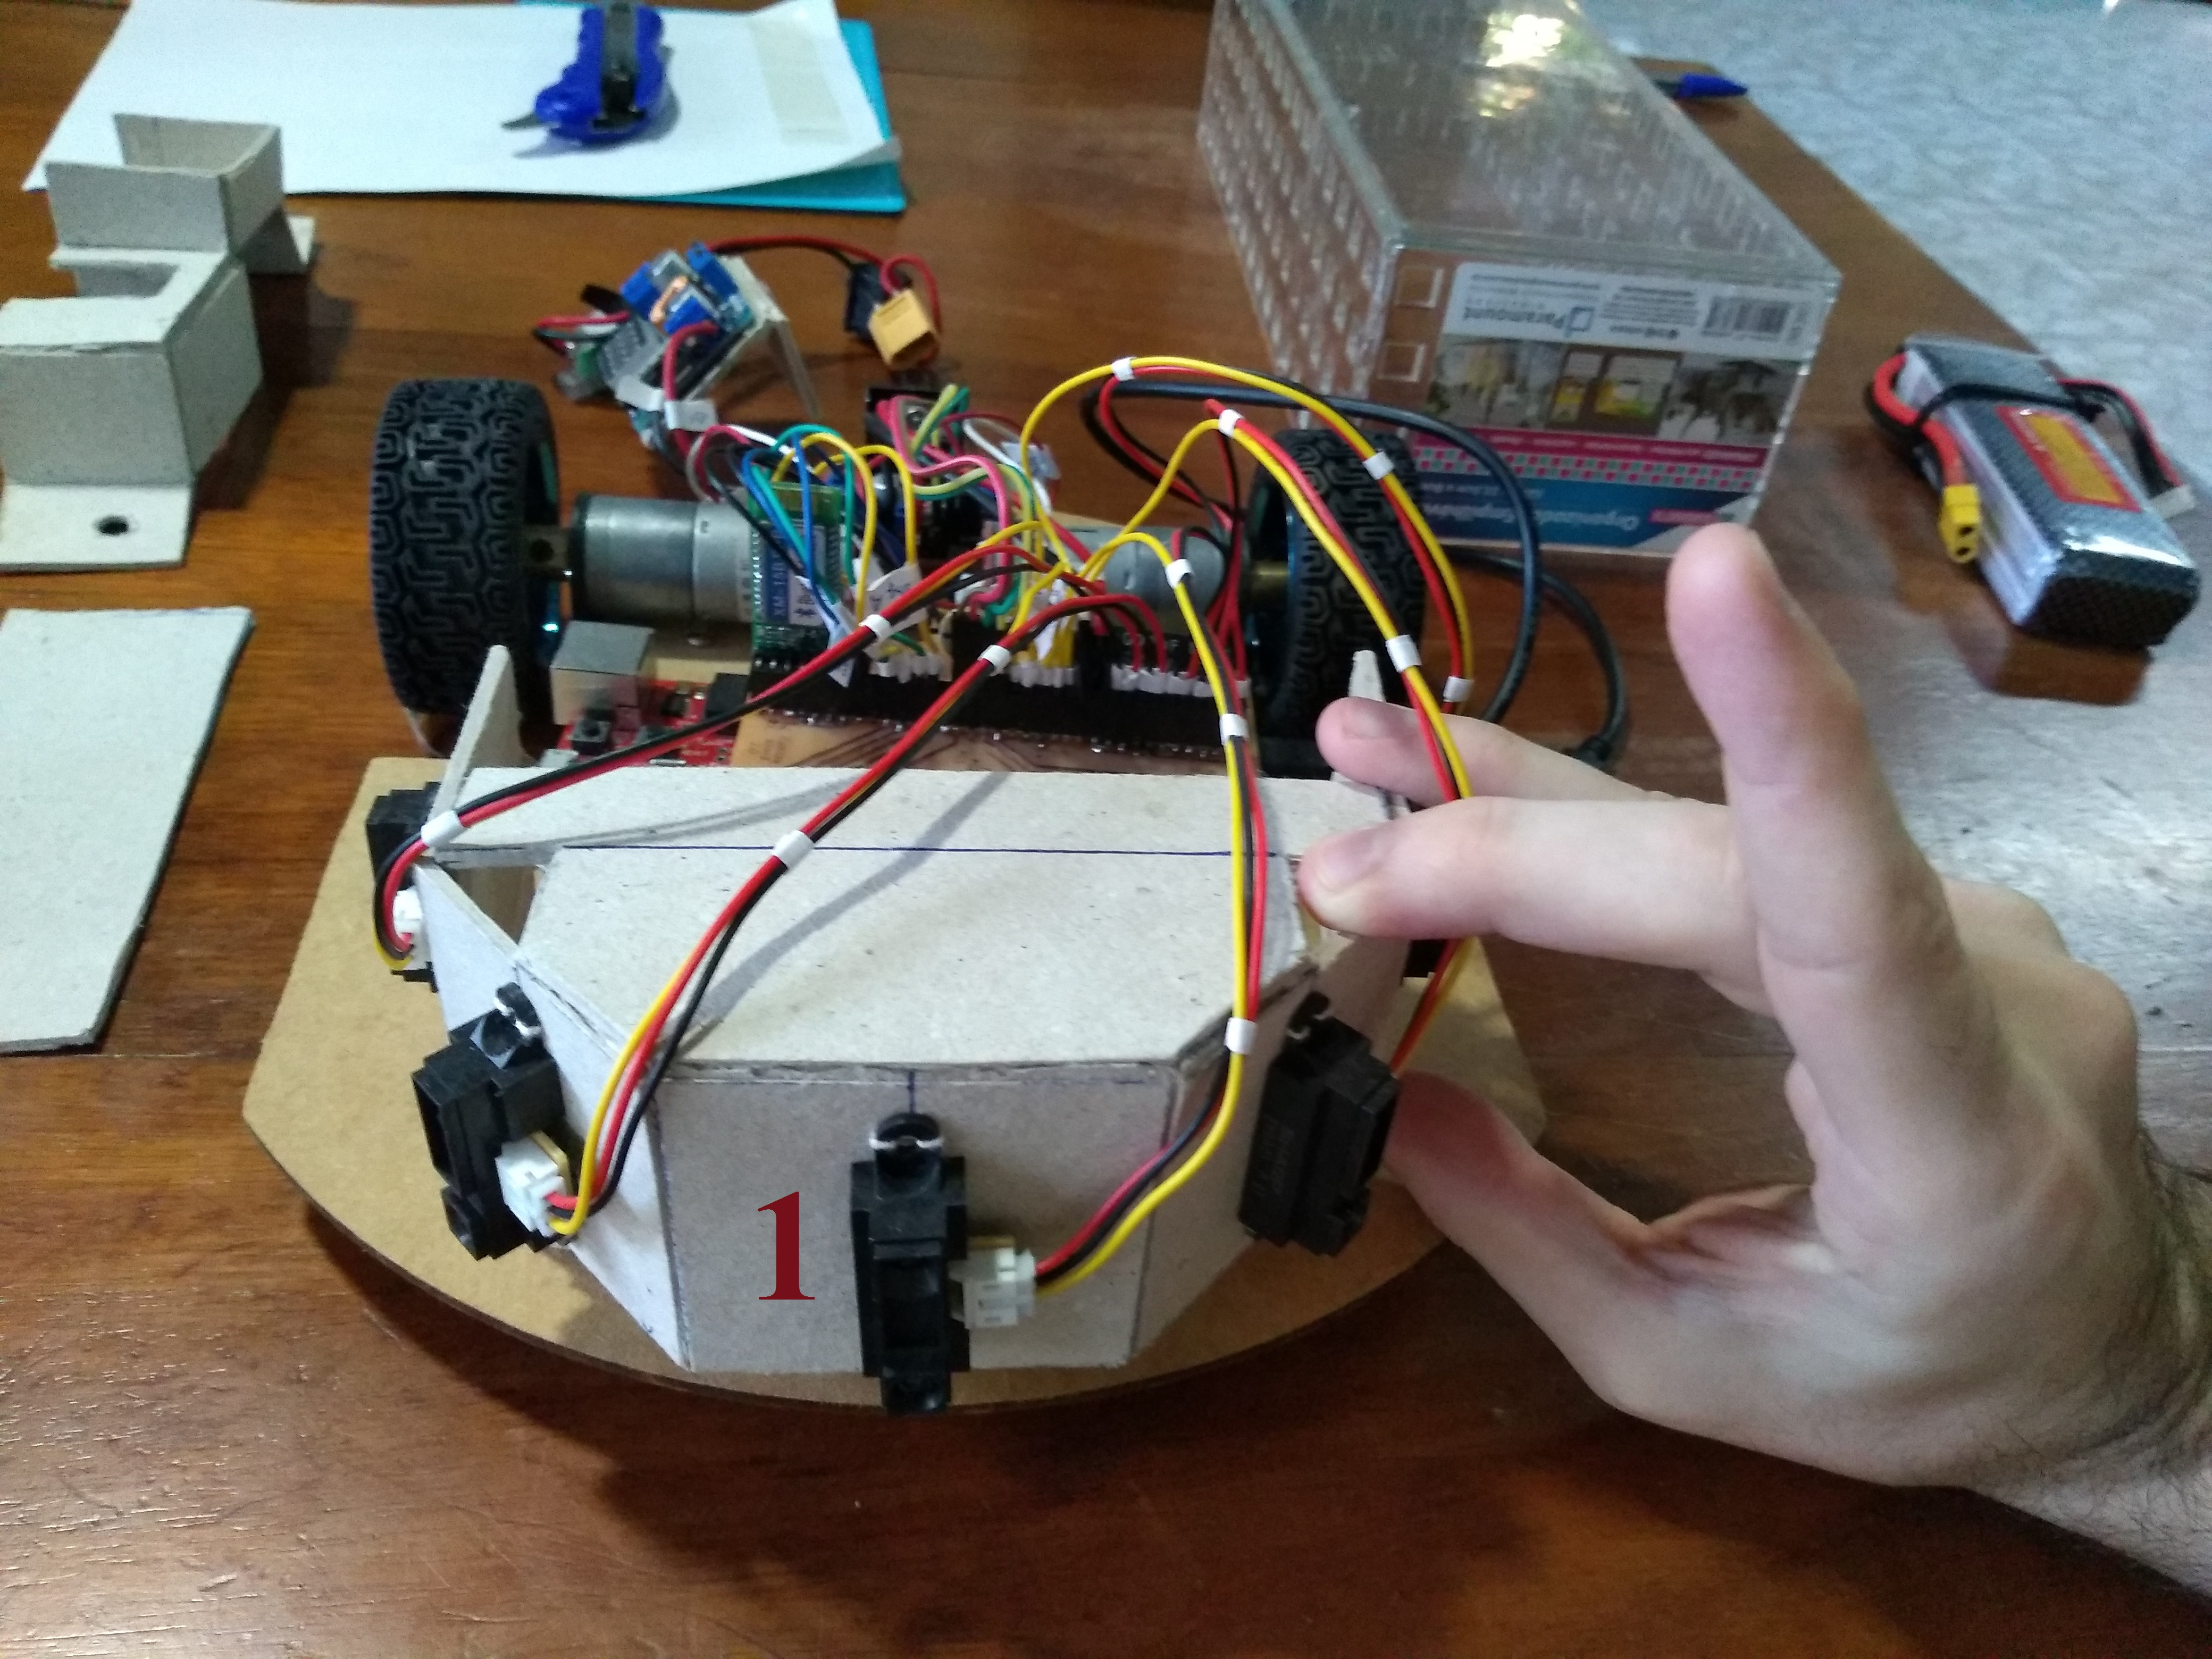
\includegraphics[trim= 0cm 0cm 0cm 0cm,clip,
scale=0.03]{Figuras/RoboMontagem1}%
		\subcaption{Posicionamento dos sensores IR}%
	\end{subfigure}%
	~
	\begin{subfigure}[b]{0.49\textwidth}%
		\centering
		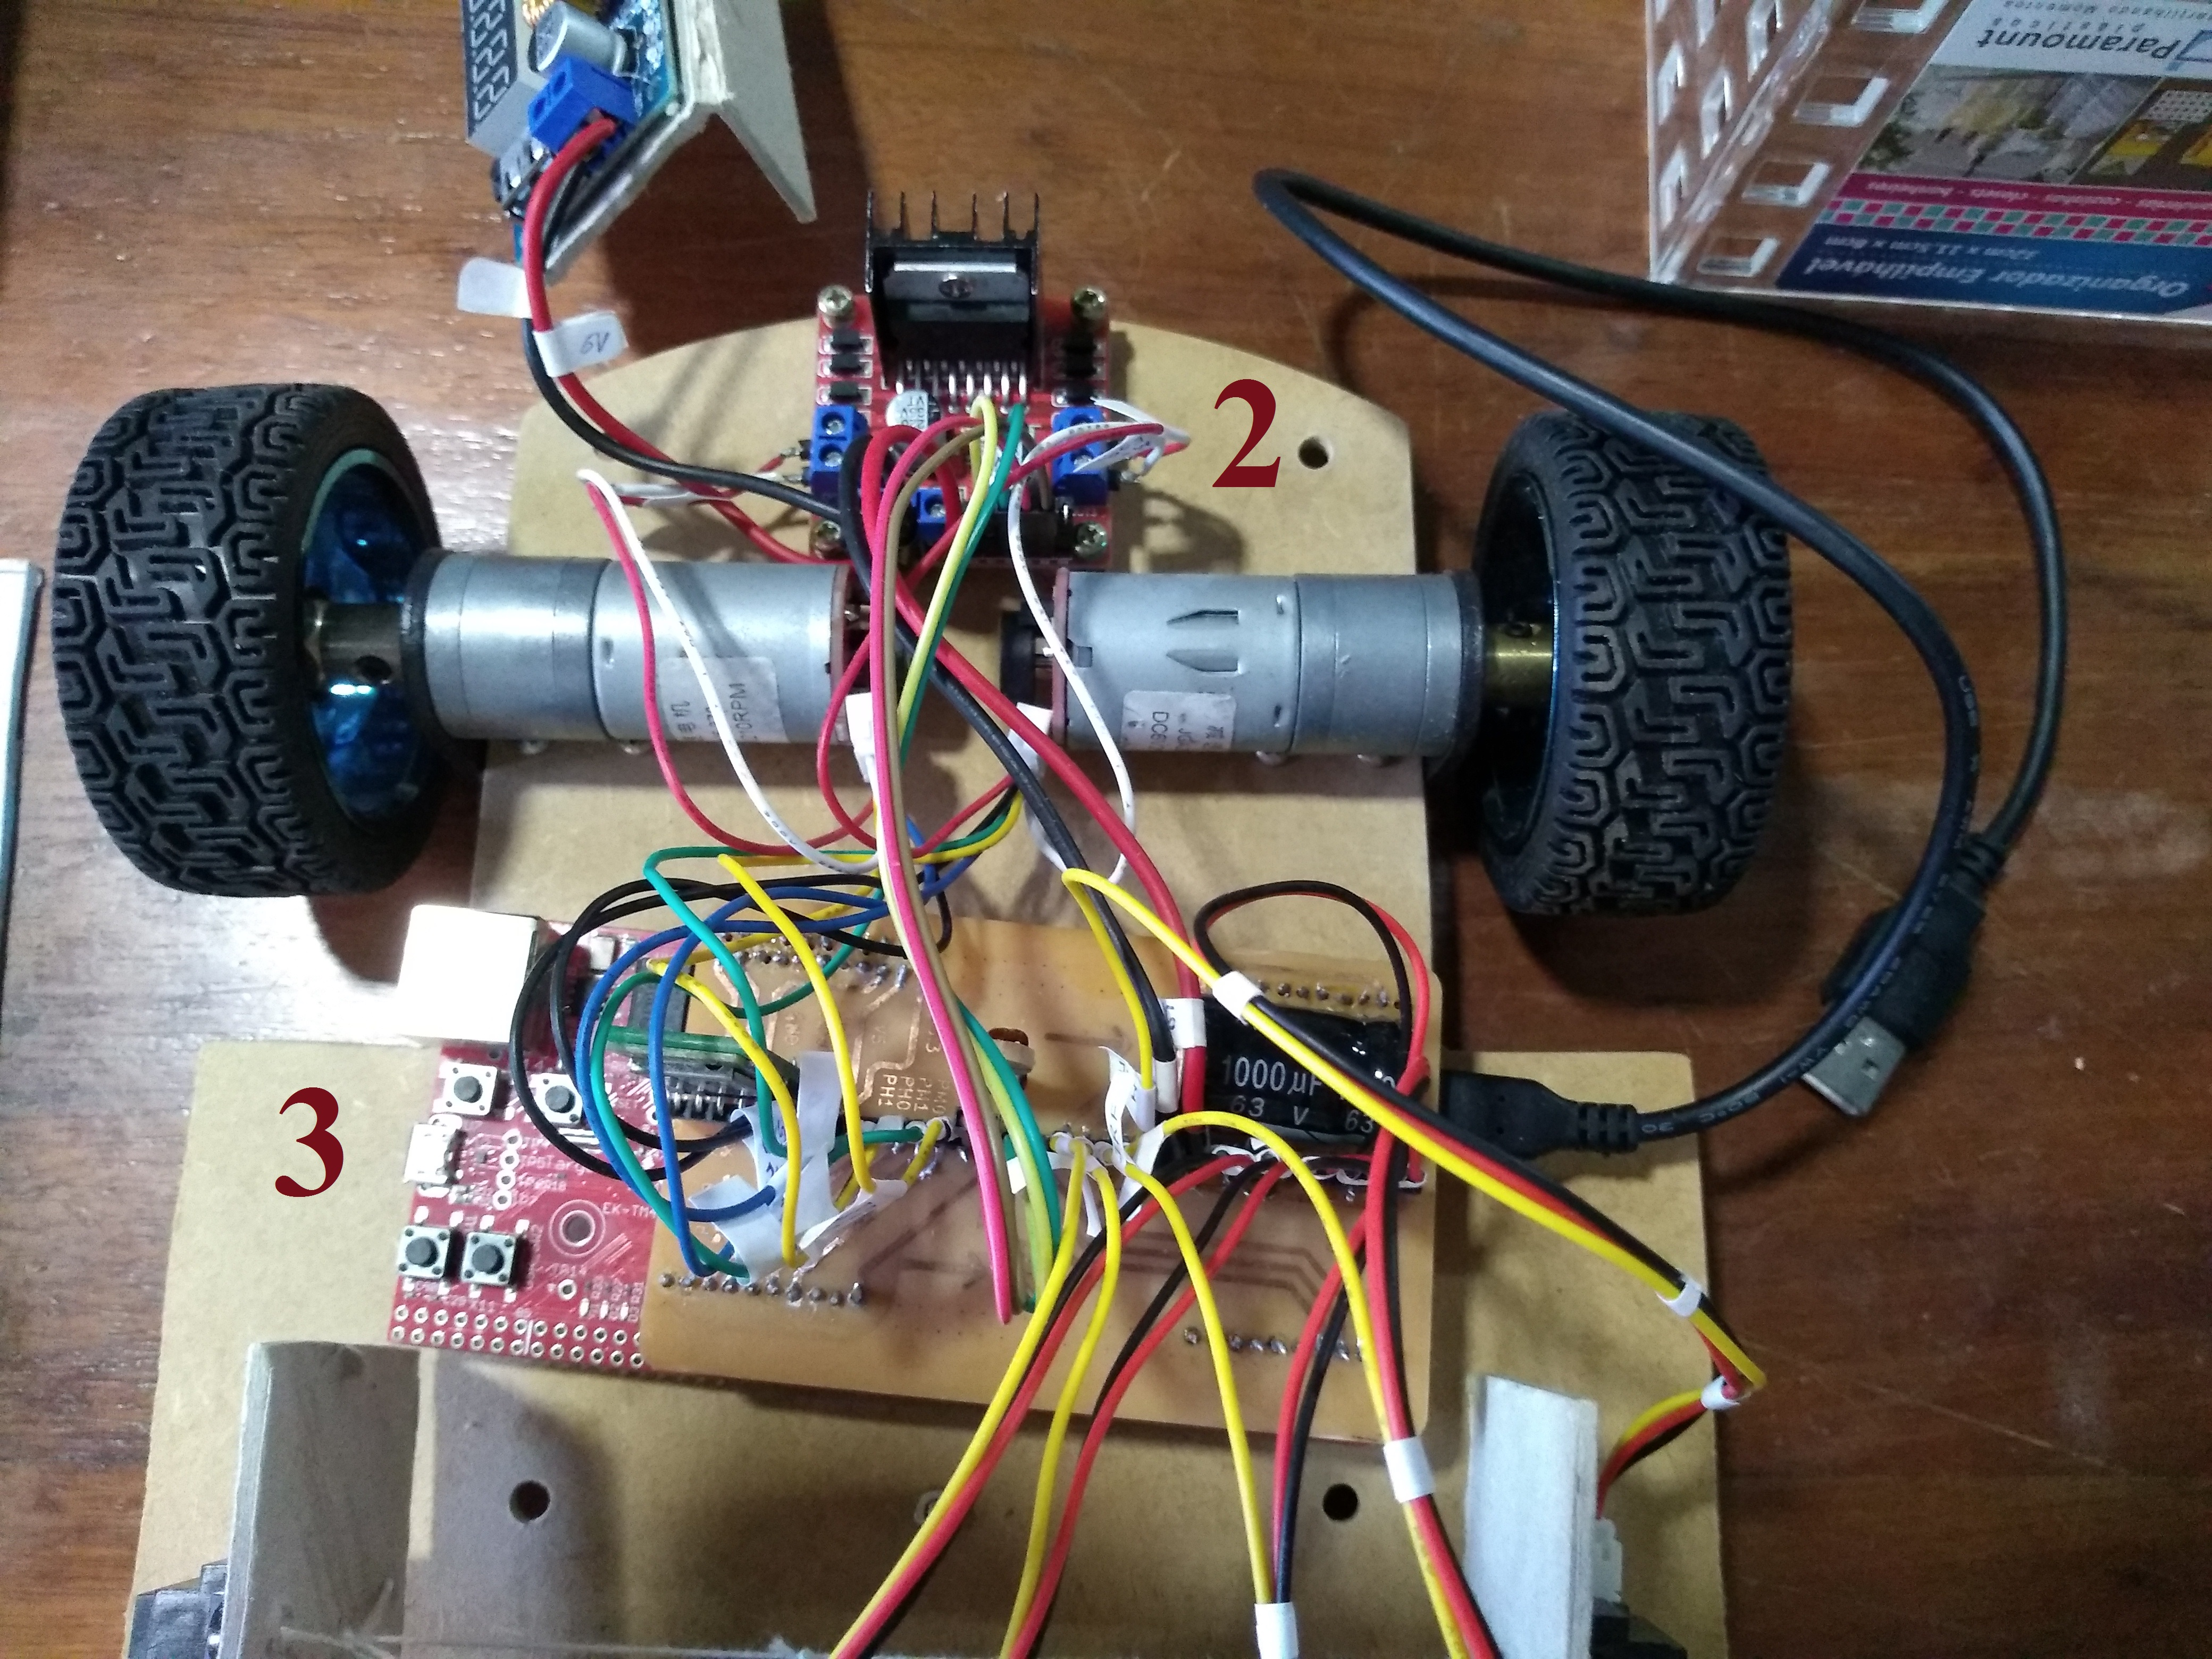
\includegraphics[trim={0cm 0cm 0cm 0cm},clip,
scale=0.03]{Figuras/RoboMontagem2}%
		\subcaption{Disposição dos motores e microcontrolador}%
	\end{subfigure}%
	~
	\begin{subfigure}[b]{0.49\textwidth}%
		\centering
		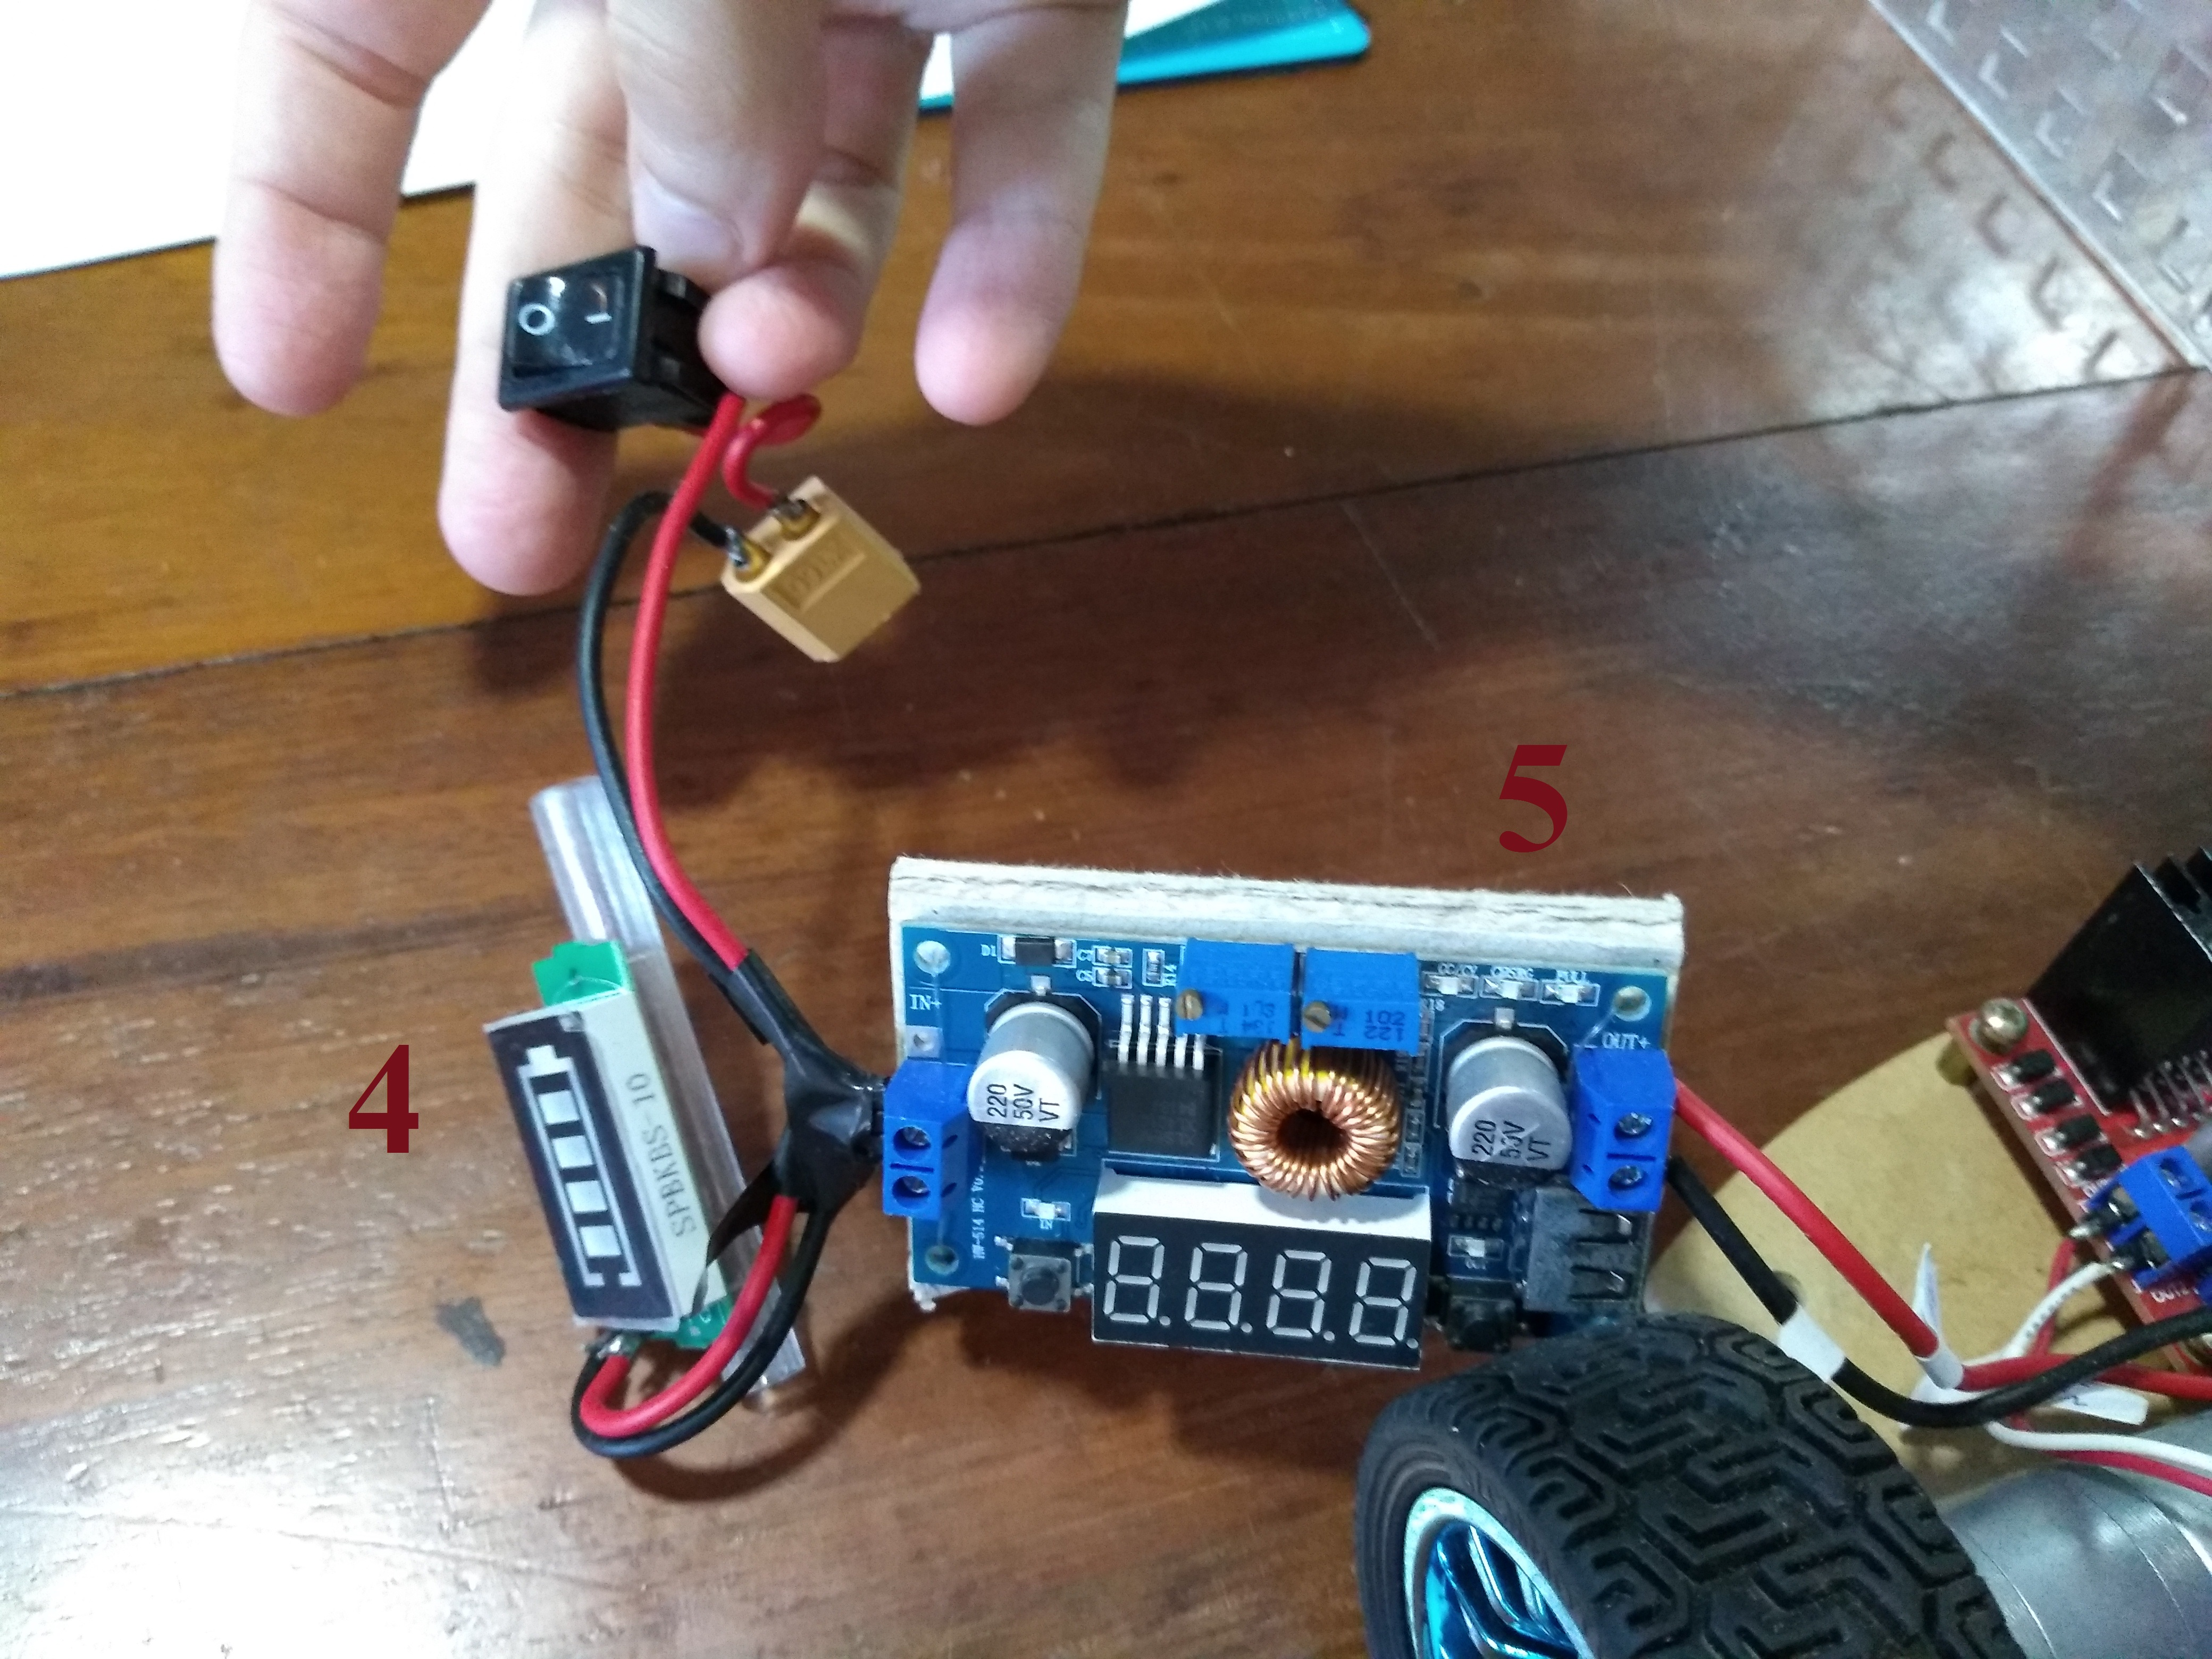
\includegraphics[trim= 0cm 0cm 0cm 0cm,clip,
scale=0.03]{Figuras/RoboMontagem3}%
		\subcaption{Regulador de Tensão}%
	\end{subfigure}%
	~
	\begin{subfigure}[b]{0.49\textwidth}%
		\centering
		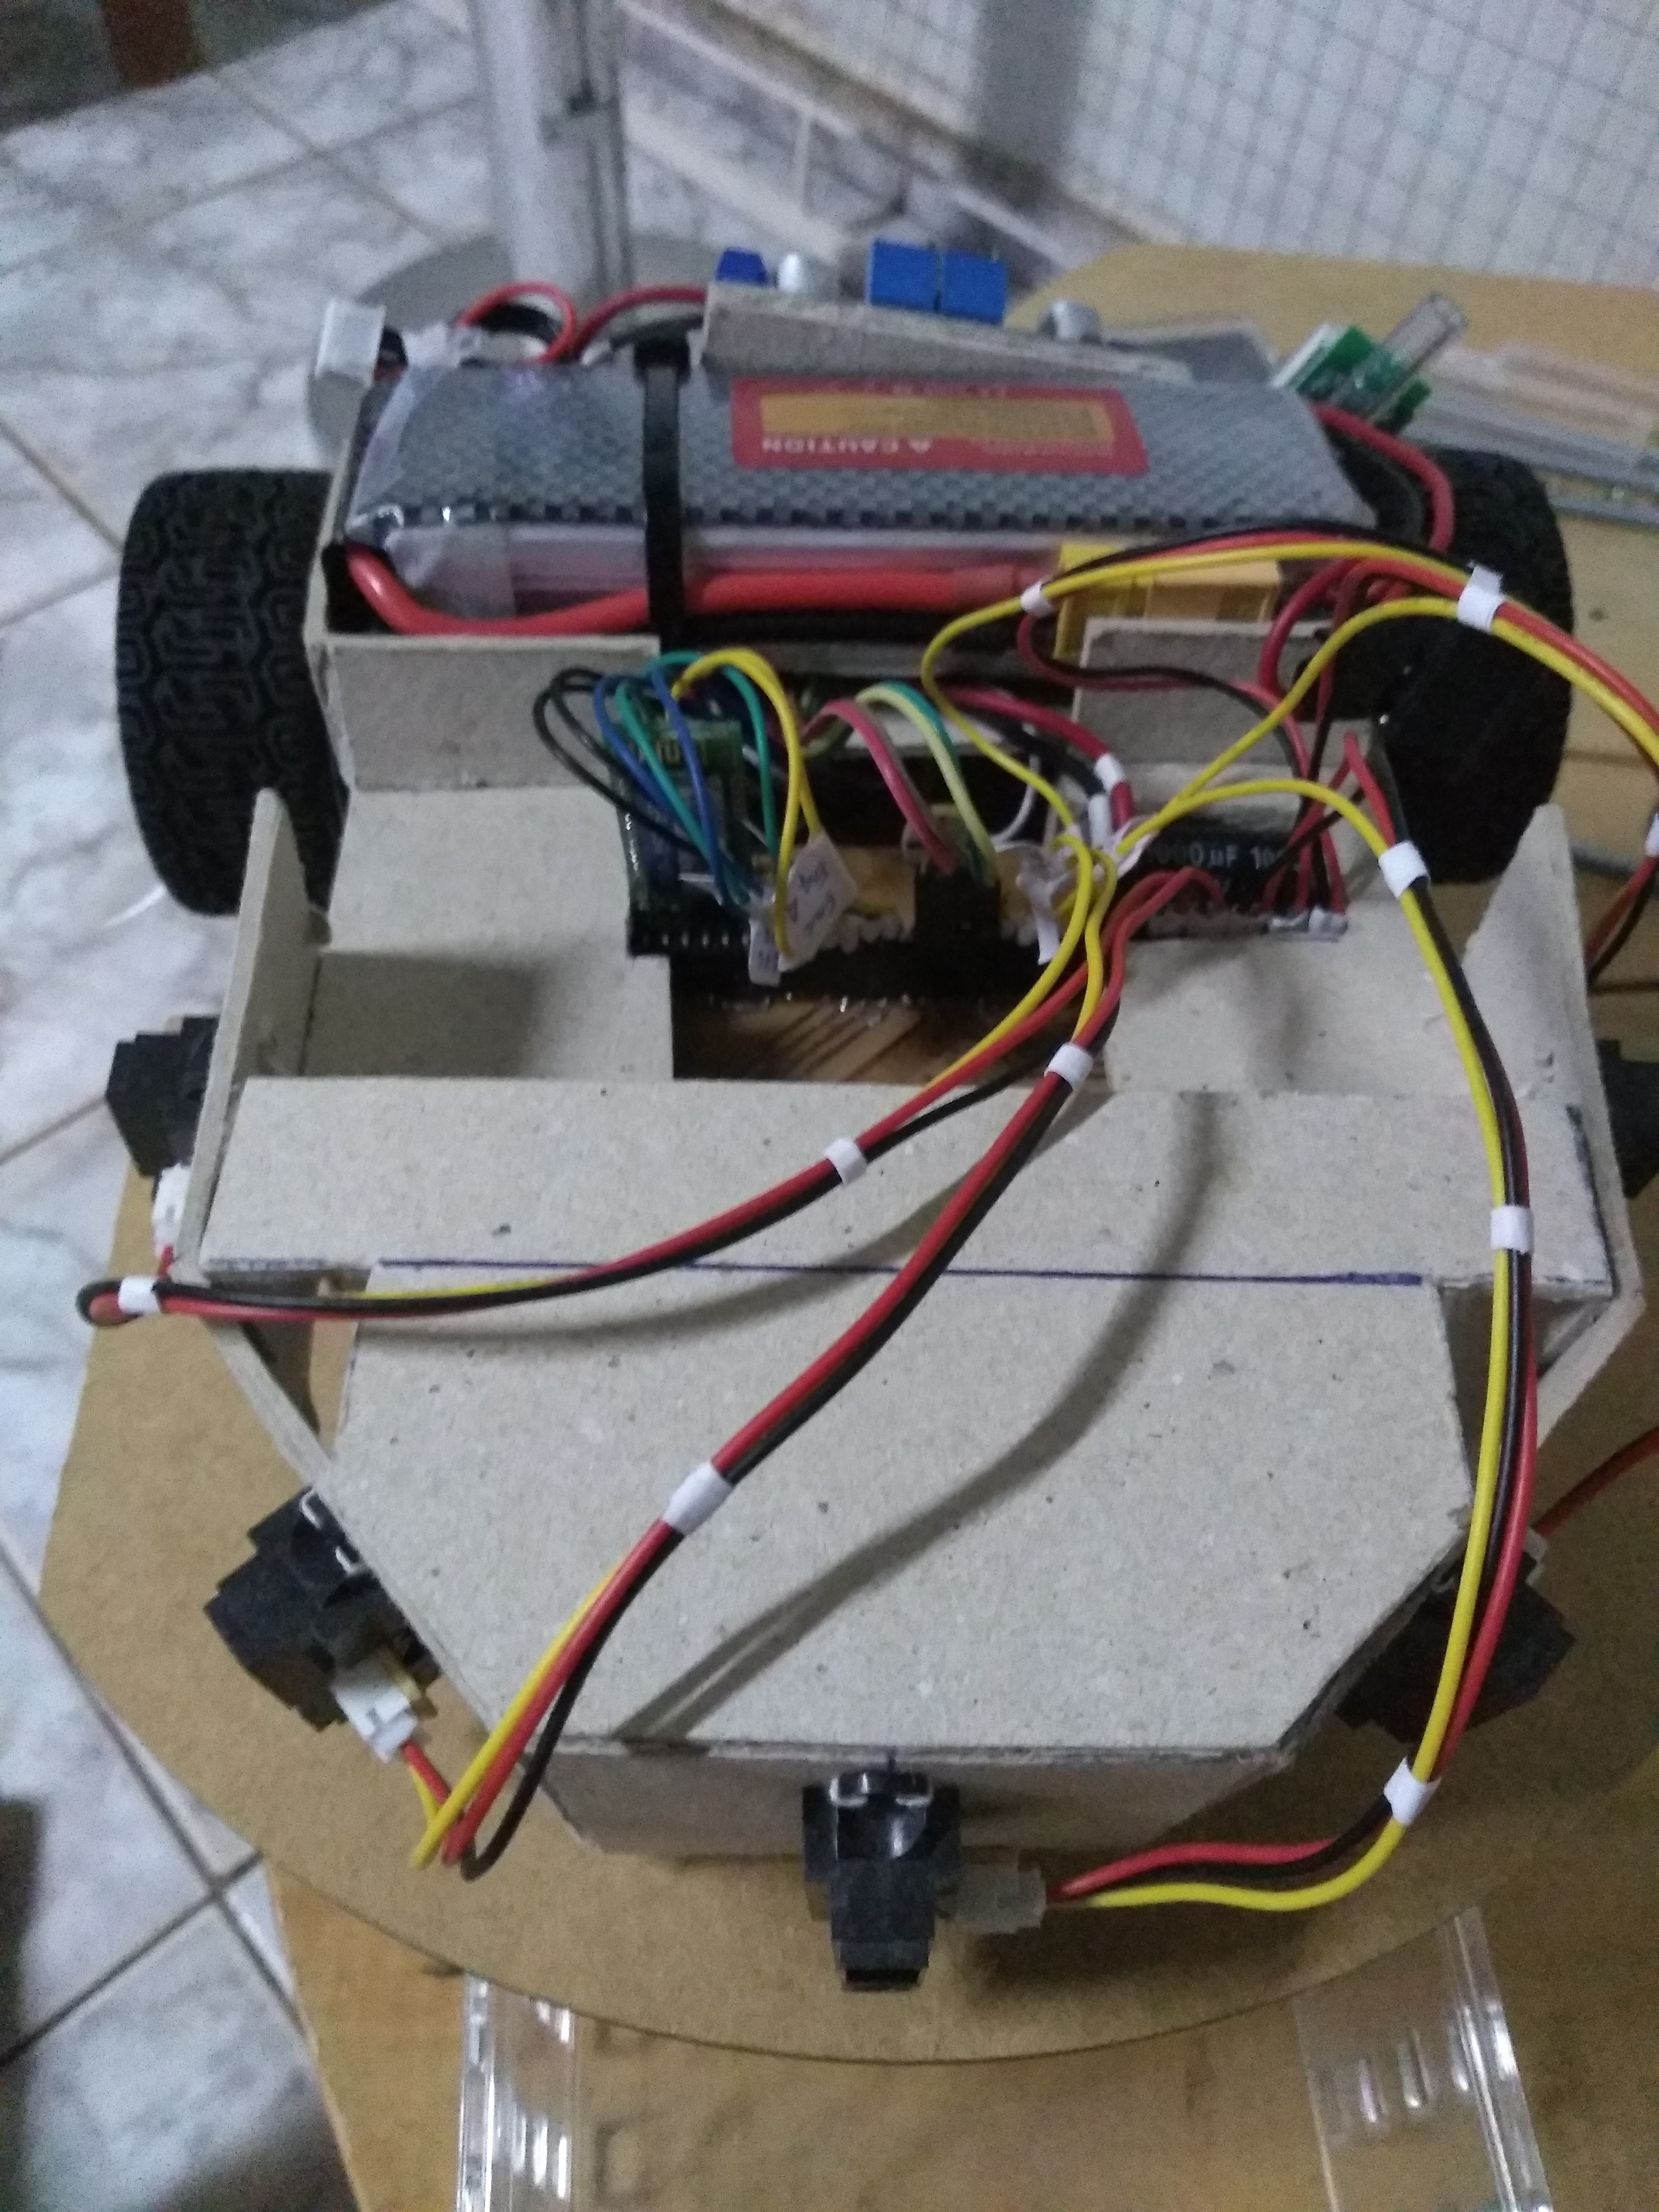
\includegraphics[trim={0cm 0cm 0cm 0cm},clip,
scale=0.03]{Figuras/RoboMontagem4}%
		\subcaption{Posicionamento dos componentes}%
	\end{subfigure}%
\end{figure}